\documentclass[10pt, a4paper]{article}


% ==> preamble
\usepackage{enumitem}
\usepackage{geometry}
\geometry{margin=0.1cm}
\pagestyle{empty}

\usepackage{tikz}
\usetikzlibrary{calc}


\def\mypic{
  \tikzpicture
  \clip (0,0) circle (2);
  \node at (0,-0.4) {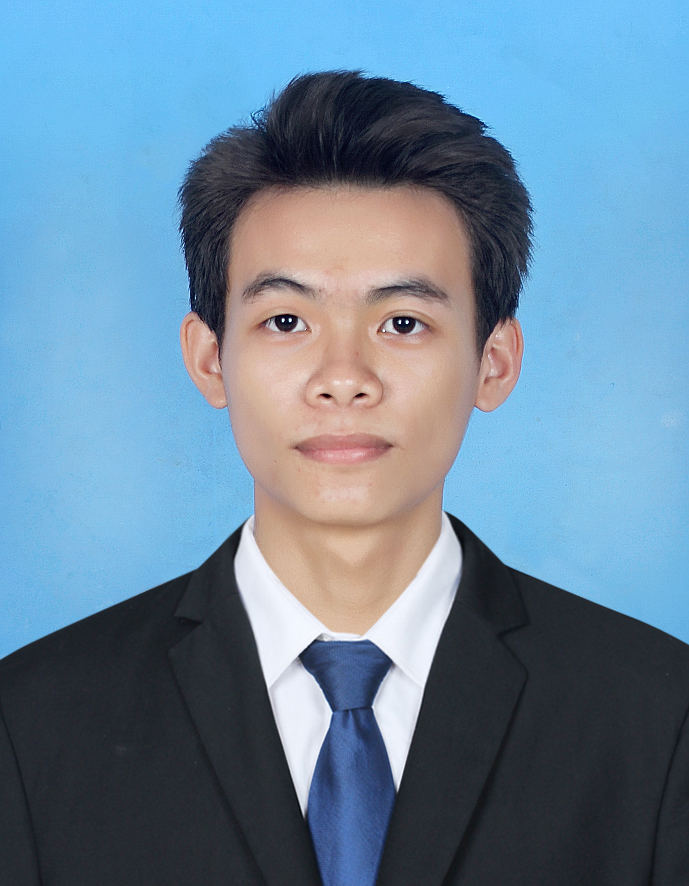
\includegraphics[scale=1.2]{me.jpg}};
  \endtikzpicture
}

\usepackage[no-math]{fontspec}
\setmainfont{Fira Sans}

\usepackage{fontawesome}
% <==
\def\mybold{\bfseries\large}
\linespread{1.2}
\usepackage{hyperref}
\hypersetup{
  colorlinks=true,
  linkcolor=magenta,
  filecolor=blue,      
  urlcolor=blue,
  pdfinfo={
    title = {Sivmeng HUN's Resume},
    author= {Sivmeng HUN}
  },
}

\def\labelitemi{{\faCaretRight}}
\def\labelitemii{{\faCaretRight}}



\def\mytitle#1{
  {
    \tikzpicture
    \draw[draw=gray] (0,0)--(10.5,0);
    \node[rectangle, draw=gray!40, inner sep=0.3cm, right,
    fill=gray!30, font=\color{black}] at (0,0) 
    {\mybold #1};
    \endtikzpicture
  }
}
\begin{document}

\begin{tikzpicture}[remember picture, overlay]

  % ==> define coordinate
  \def\wx{8cm}
  \def\wy{6.4cm}
  \def\margin{1cm}
  \coordinate (A) at (current page.north west);
  \coordinate (B) at (current page.north east);
  \coordinate (C) at (current page.south east);
  \coordinate (D) at (current page.south west);

  \coordinate (E) at ($(current page.north west)+(\wx,0)$);
  \coordinate (F) at ($(current page.south west)+(\wx,0)$);
  \coordinate (G) at ($(current page.north west)+(0,-\wy)$);
  \coordinate (H) at ($(current page.north east)+(0,-\wy)$);
  % <==
  % ==> me and my name
  \draw[gray] (E)--(F);
  \node[scale=1.2] (mypic) at ($(A)+(\wx/2, -\wy/2)$) {\mypic};
  \node[xshift=\margin, yshift=-1cm, font=\huge, right] at (G) {HUN Sivmeng};
  %\node[yshift=-5cm, font=\bfseries\huge] at (mypic) {HUN Sivmeng};
  %\draw[help lines] (A)--(G)--(H)--(B)--cycle;
  % <==
  % ==> left side
  \node[
    rectangle, anchor=north west,
    text width=6cm, text badly ragged
    ] at ($(G)+(\margin, -3cm)$)
    {
      % ==> personal info
      {\mybold Personal Info}\\
      \begin{itemize}
        \item[\faHome] Phnom Penh | Cambodia
        \item[\faCalendar] 27 September | 2003
        \item[\faGraduationCap] RUPP | Maths | 3\textsuperscript{rd} year
        \item[\faGlobe] Language
          \begin{itemize}
            \item Khmer (native)
            \item English (elementary)
          \end{itemize}
      \end{itemize}
      \vspace{1cm}
      % <==
      % ==> contact info
      {\mybold Contact}\\
      \begin{itemize}
        \item[\faEnvelope] {\href{mailto://mengsivmeng@gmail.com}{\ttfamily mengsivmeng@gmail.com}}
        \item[\faPhoneSquare] {\href{phone}{\ttfamily (+855) 31 749 5858}}
        \item[\faFacebookSquare] {\url{fb.com/meng.sivmeng.er}}
        \item[\faPaperPlane] {\url{t.me/meng_sivmeng}} 
        \item[\faGithub] {\url{github.com/mengistic}}
      \end{itemize}
      \vspace{1cm}
      % <==
      % ==> hobbies
      {\mybold Hobbies}\\
      Read math books | Watching lecture notes | 
      Programming | mozart | chess | movies | anime | coffee
      % \begin{itemize}
      %   \item Reading math books 
      %   \item watching lecture notes on Youtube
      %   \item Streaming movies
      %   \item Ricing Linux
      %   \item Hanging out with friends
      % \end{itemize}
      % <==

    };
  % <==
  \node[
    rectangle, anchor=north west,
    text width=10.5cm, text badly ragged
    ] at ($(E)+(\margin, -1cm)$) {

      % ==> education and awards
      \mytitle{\faGraduationCap~~Education and Achievement}
      \begin{itemize}[label={}, leftmargin=0mm]
        % ==> 2017-2020
        \item {\bfseries 2017--2020}\\
          \begin{itemize}
            \item Entered Hun Sen Highschool of Kamchaymear
            \item Was a 5\textsuperscript{th} ranking candidate in 
              {\itshape Cambodian Outstanding Student Competition 
              (Grade 9)} for mathematics in national round 
            \item Won two gold medals from two distinct mathematical
              competitions (WMI and SASMO)
          \end{itemize}
          % <==
          % ==> 2020
        \item {\bfseries 2020}\\
          \begin{itemize}
            \item 
              Was trained for {\itshape International Mathematical Olympiad} 
              (IMO) at RUPP for 3 months
            \item Completed a level 9 English program 
              at {Pannasastra} University of Cambodia (PUC)
          \end{itemize}
          % <==
          
        \item {\bfseries 2020--2022}
          \begin{itemize}
          \item Enter Royal University of Phnom Penh (RUPP)
          \item Achieved an overall GPA of 3.91 (1\textsuperscript{st} year)
          \item Achieved an overall GPA of 3.80 (2\textsuperscript{nd} year)
          \item Was selected for a mentoring program in Mathematics by
            {\itshape Forum for Pushing the Boundary} (FPB)
          \item Attended {\itshape in Summer School on Algorithms and Programming in
            Python}, by professors \textit{Roberto Mantaci} and \textit{Jean-Baptiste Yunes}.
          \item Attended in {\itshape Data Analytics Camp}, 2023 Unitwin, by
            Doctors \textit{Daiyon Cho} and \textit{Dim Dae Shik}.
          \end{itemize}
      \end{itemize}
      \vspace{0.4cm}
      % <==
      % ==> skills

      \mytitle{\faSuperscript~~Maths}
      \begin{itemize}
      \item {\bfseries Studied}
        Linear Algebra | Real Analysis | Abstract Algebra |
        Number Theory | Complex Analysis
      \item {\bfseries Studying}
        Algebraic Geometry | Differential Geometry |
        Dynamical System | Topology | Vector Calculus |
        Functional Analysis
      \end{itemize}
      
      \mytitle{\faTags~~Others}
      \begin{itemize}
        \item[\faTerminal] 
          {\bfseries Programming (basics): } 
          Sage | R  | LaTeX | C |  C++ |  Python |  Javascript |
          Asymptote 
        \item[\faStackOverflow]
          {\bfseries Technology: }
          Linux | Emacs | Vim | Emacs | Command line | Git
      \end{itemize}
      \vspace{0.3cm}
      % <==
      % ==> ref
      \mytitle{\faPaperclip~~Reference}
      \begin{itemize}
      \item[\faUser] Professor \textit{Rod Halburd}
        \href{mailto://r.halburd@ucl.ac.uk}{\ttfamily r.halburd@ucl.ac.uk}
      \end{itemize}
      % <==

    };



\end{tikzpicture}


\end{document}
